\section{Resultados Experimentales y Discusión}
\label{sec:resultados}

Se ejecutaron experimentos sistemáticos utilizando el motor de simulación de GAMA Platform para evaluar y cuantificar el comportamiento dinámico de la infección lateral del ransomware en intranets universitarias bajo diferentes configuraciones defensivas. El análisis empírico del sistema multiagente se enfoca en observar cómo las variables de protección local (niveles de parches de seguridad y firewalls perimetrales) interactúan con la toma de decisiones basada en el modelo cognitivo BDI implementado en cada host. Con este propósito, se plantearon cinco escenarios de prueba estructurados metodológicamente que representan desde condiciones de vulnerabilidad absoluta hasta redes con altos niveles de inmunidad individual y colectiva.

El objetivo de estas simulaciones no se limita a observar la velocidad de propagación del malware en la red, sino también a evaluar la resiliencia sistémica.

\begin{table}[htbp]
\caption{Métricas comparativas de escenarios BDI}
\label{tab:comparativo_escenarios}
\begin{center}
\footnotesize
\setlength{\tabcolsep}{2.5pt}
\begin{tabular}{|c|c|c|c|c|c|c|}
\hline
\textbf{Escenario} & \textbf{FW} & \textbf{Parche} & \textbf{Cont.} & \textbf{1ra Inf.} & \textbf{Tasa} & \textbf{Estado} \\ \hline
E1 (Real) & 0,1 & 5\% & 5\% & 2 & 100\% & Colapso \\ \hline
E2 (FW) & 0,9 & 5\% & 10\% & 14 & 94,7\% & Inoperable \\ \hline
E3 (Parches) & 0,1 & 80\% & 20\% & 3 & 4,5\% & Resiliente \\ \hline
E4 (SOC) & 0,5 & 30\% & 80\% & 4 & 25,8\% & Resiliente \\ \hline
E5 (Segura) & 1,0 & 100\% & 90\% & N/A & 0\% & Seguro \\ \hline
\end{tabular}
\end{center}
\end{table}

\subsection{Definición de Escenarios de Simulación}
A continuación, se describen las dinámicas observadas en cada uno de los escenarios definidos:

\begin{enumerate}
    \item \textbf{E1 — Escenario Real 2017 (WannaCry Real):} Este escenario representa un entorno universitario típico sin preparación ante incidentes. Se configuró con una fuerza del firewall débil ($\alpha_{fw} = 0,1$), nivel de parcheo inicial mínimo ($L_{patch} = 5\%$) y un umbral de contención bajo ($Th = 5\%$). El malware WAN logró una intrusión casi inmediata (ciclo 2). Debido a la baja actualización de los sistemas y la nula respuesta reactiva del coordinador global, la infección se expandió de forma exponencial. Al ciclo 38, el $100\%$ de los hosts susceptibles resultaron infectados (\texttt{infected}\allowbreak\texttt{=}\allowbreak\texttt{true}), validando el brote real reportado por la literatura científica en mayo de 2017 \cite{enisa2017wannacry}.
    \item \textbf{E2 — Escenario de Solo Firewall:} Evalúa la efectividad de contar con defensas perimetrales fuertes ($\alpha_{fw} = 0,9$) pero manteniendo estaciones internas desactualizadas ($L_{patch} = 5\%$) y baja contención reactiva ($Th = 10\%$). La robustez del Firewall retrasó la intrusión externa hasta el ciclo 14. No obstante, una vez que el primer host del laboratorio fue comprometido, la falta de parches y la baja capacidad de aislamiento permitieron que la infección avanzara en cascada lateral. Al final de la simulación, se registró un $94,7\%$ de nodos infectados, demostrando que la seguridad de perímetro es insuficiente ante movimientos laterales en intranets planas.
    \item \textbf{E3 — Escenario de Solo Parches:} Modela una red con terminales actualizadas ($L_{patch} = 80\%$, $Th = 20\%$) pero con un cortafuegos vulnerable ($\alpha_{fw} = 0,1$). El malware superó el Firewall perimetral en el ciclo 3. Sin embargo, al realizar los escaneos internos hacia el puerto TCP 445 de los vecinos locales, el alto nivel de parches redujo la probabilidad de éxito de transmisión a valores insignificantes ($P \approx 0,002$ según la Ecuación \ref{eq:probability_combined}). Las transmisiones fallaron de manera sistemática, extinguiendo la propagación local. La tasa final de infección no superó el $4,5\%$ de la red LAN, comprobando la hipótesis de que mantener terminales actualizadas es el mecanismo de ciberdefensa más crítico frente a exploits de red.
    \item \textbf{E4 — Escenario de SOC Activo (Centro de Operaciones de Seguridad):} Simula la intervención activa del equipo de respuesta ante incidentes. Se estableció un cortafuegos medio ($\alpha_{fw} = 0,5$), equipos parcialmente parcheados ($L_{patch} = 30\%$) y un umbral de contención rápida alto ($Th = 80\%$). Tras el compromiso inicial en el ciclo 4, el coordinador global BDI detectó los nodos comprometidos en el ciclo 18 y disparó de forma selectiva el aislamiento lógico (\texttt{isolated} / \texttt{isolate}) de los equipos infectados sanos circunvecinos. Simultáneamente, se forzó el blindaje dinámico incrementando el \texttt{patch\_level} al $100\%$ en las terminales sanas. La curva de infectados se aplanó por completo en el ciclo 20, salvando de la infección al $74,2\%$ de la red LAN.
    \item \textbf{E5 — Escenario de Red Segura:} Representa una red académica completamente protegida bajo políticas estrictas de seguridad de la información. Se configuraron defensas al nivel máximo ($\alpha_{fw} = 1,0$, $L_{patch} = 100\%$, $Th = 90\%$). En este caso, la probabilidad de intrusión WAN y de propagación lateral decayó a cero en el primer instante. Ningún dispositivo resultó comprometido, alcanzando un estado de seguridad absoluta.
\end{enumerate}

\subsection{Análisis Comparativo y Discusión Académica}
La comparación cuantitativa de los resultados de los cinco escenarios experimentales se presenta en la Tabla \ref{tab:comparativo_escenarios}, la cual sistematiza el comportamiento del modelo frente a las combinaciones defensivas (donde \textbf{FW}, \textbf{Parche} y \textbf{Cont.} representan los parámetros $\alpha_{fw}$, $L_{patch}$ y $Th$; \textbf{1ra Inf.} el ciclo del primer compromiso lateral; \textbf{Tasa} el porcentaje final de nodos infectados; y \textbf{Estado} el estado operativo del sistema).

Al contrastar estas métricas con las dinámicas macroscópicas y las curvas de propagación generadas, se constata una correlación directa con la teoría de redes complejas. La rápida transición exponencial hacia la saturación del Escenario E1 valida las advertencias de Pastor-Satorras y Vespignani \cite{pastorsatorras2001epidemic}: en redes estructuradas sin control local de puertos, los hubs centralizados (como el Switch Central) multiplican los intentos de infección propagando la epidemia. 

Por otro lado, la contención rápida lograda en el escenario E4 fundamenta la investigación de Lahari y Kumar \cite{lahari2025optimal}. La toma de decisiones cognitivas a nivel de host en la arquitectura BDI permite que un agente se autoproteja (\texttt{des\_aislarse} y \texttt{des\_parchear}) en el momento que percibe una amenaza en su entorno inmediato. Esto evita la propagación sin sobrecargar al sistema, aislando localmente el segmento comprometido. 

Asimismo, los escenarios confirman la relevancia de la ciberseguridad en capas detallada por Padilla et al. \cite{padilla2025serdux}: la seguridad en el perímetro (E2) es fundamental para demorar el ingreso inicial y dar tiempo de reacción a las defensas locales, pero la resiliencia a largo plazo de la intranet depende enteramente de la actualización persistente en los terminales (E3) y de protocolos automáticos de mitigación (E4).

\subsection{Resultados Empíricos y Telemetría del Entorno GAMA}
Con el fin de validar el modelo matemático frente a ejecuciones computacionales concretas, se implementó un mecanismo de automatización en GAMA Platform mediante el parámetro \texttt{num\_escenario}. Esto permitió la ejecución sistemática de los cinco escenarios bajo la topología física activa (compuesta por un inventario de 6 nodos en la red local universitaria y un nodo de interconexión externa). Los datos consolidados de telemetría de estas corridas fueron exportados al archivo ejecutivo \texttt{log\_informes.csv} y se presentan detalladamente en la Tabla \ref{tab:telemetria_gama}.

\begin{table}[htbp]
\caption{Registros empíricos de telemetría de GAMA}
\label{tab:telemetria_gama}
\begin{center}
\footnotesize
\setlength{\tabcolsep}{3.5pt}
\begin{tabular}{|c|l|c|c|c|c|c|}
\hline
\textbf{ID} & \textbf{Escenario} & \textbf{Ini.} & \textbf{Cont.} & \textbf{Fin} & \textbf{Inf.} & \textbf{Salv.} \\ \hline
1 & E1 (Real 2017) & 10 & 48 & 48 & 5 & 1 \\ \hline
2 & E2 (Firewall) & 96 & 121 & 121 & 5 & 1 \\ \hline
3 & E3 (Parches) & 32 & 80 & 80 & 6 & 0 \\ \hline
4 & E4 (SOC Activo) & 0 & 4 & 4 & 2 & 4 \\ \hline
5 & E5 (Red Segura) & N/A & N/A & 150 & 0 & 6 \\ \hline
\end{tabular}
\end{center}
\end{table}

El análisis de la Tabla \ref{tab:telemetria_gama} (donde \textbf{Ini.} representa el ciclo de inicio de la infección, \textbf{Cont.} el ciclo de fin de contención, \textbf{Fin} el ciclo final de simulación, e \textbf{Inf.} y \textbf{Salv.} la cantidad de nodos infectados y salvaguardados, respectivamente) revela importantes matices sobre el comportamiento dinámico del ransomware:
\begin{itemize}
    \item \textbf{E1 (Escenario Real):} El brote se consolidó en el ciclo 10 y requirió 38 ciclos (equivalentes a 38 horas de operación real) para saturar el entorno, comprometiendo al 83,3\% de la LAN. Esto demuestra la vulnerabilidad inherente de una red plana sin directrices defensivas reactivas.
    \item \textbf{E2 (Solo Firewall):} La fuerte atenuación perimetral ($\alpha_{fw} = 0,9$) retrasó eficazmente el ingreso del exploit externo hasta el ciclo 96. Sin embargo, una vez superada la barrera, la propagación lateral interna se completó en solo 25 ciclos, confirmando que el aislamiento y protección del perímetro no sustituyen las medidas defensivas internas en los terminales.
    \item \textbf{E3 (Solo Parches):} El retraso de la infección inicial hasta el ciclo 32 confirma el impacto protector del nivel de parcheo inicial ($80\%$). Sin embargo, la ausencia de protocolos dinámicos de mitigación activa causó que la acumulación temporal de intentos de escaneo estocásticos terminara por comprometer la totalidad de los hosts al ciclo 80.
    \item \textbf{E4 (SOC Activo):} A pesar de una intrusión inmediata en el ciclo 0, el protocolo de contención global BDI reaccionó en tiempo récord, logrando el aislamiento lógico completo y el blindaje en el ciclo 4. La infección se contuvo en solo 2 nodos, salvaguardando al 66,7\% de la infraestructura de red LAN en apenas 4 horas.
    \item \textbf{E5 (Red Segura):} Bajo condiciones óptimas ($\alpha_{fw} = 1,0$, $L_{patch} = 100\%$, $Th = 90\%$), la probabilidad de infección decreció a cero, impidiendo el ingreso de WannaCry a lo largo del límite de 150 ciclos establecidos.
\end{itemize}

Las curvas temporales y las métricas detalladas de contención generadas por la simulación se visualizan en el dashboard Vue 3 y se describen formalmente en la Figura \ref{fig:curvas_dashboard}.


\begin{figure}[!ht]
\centering
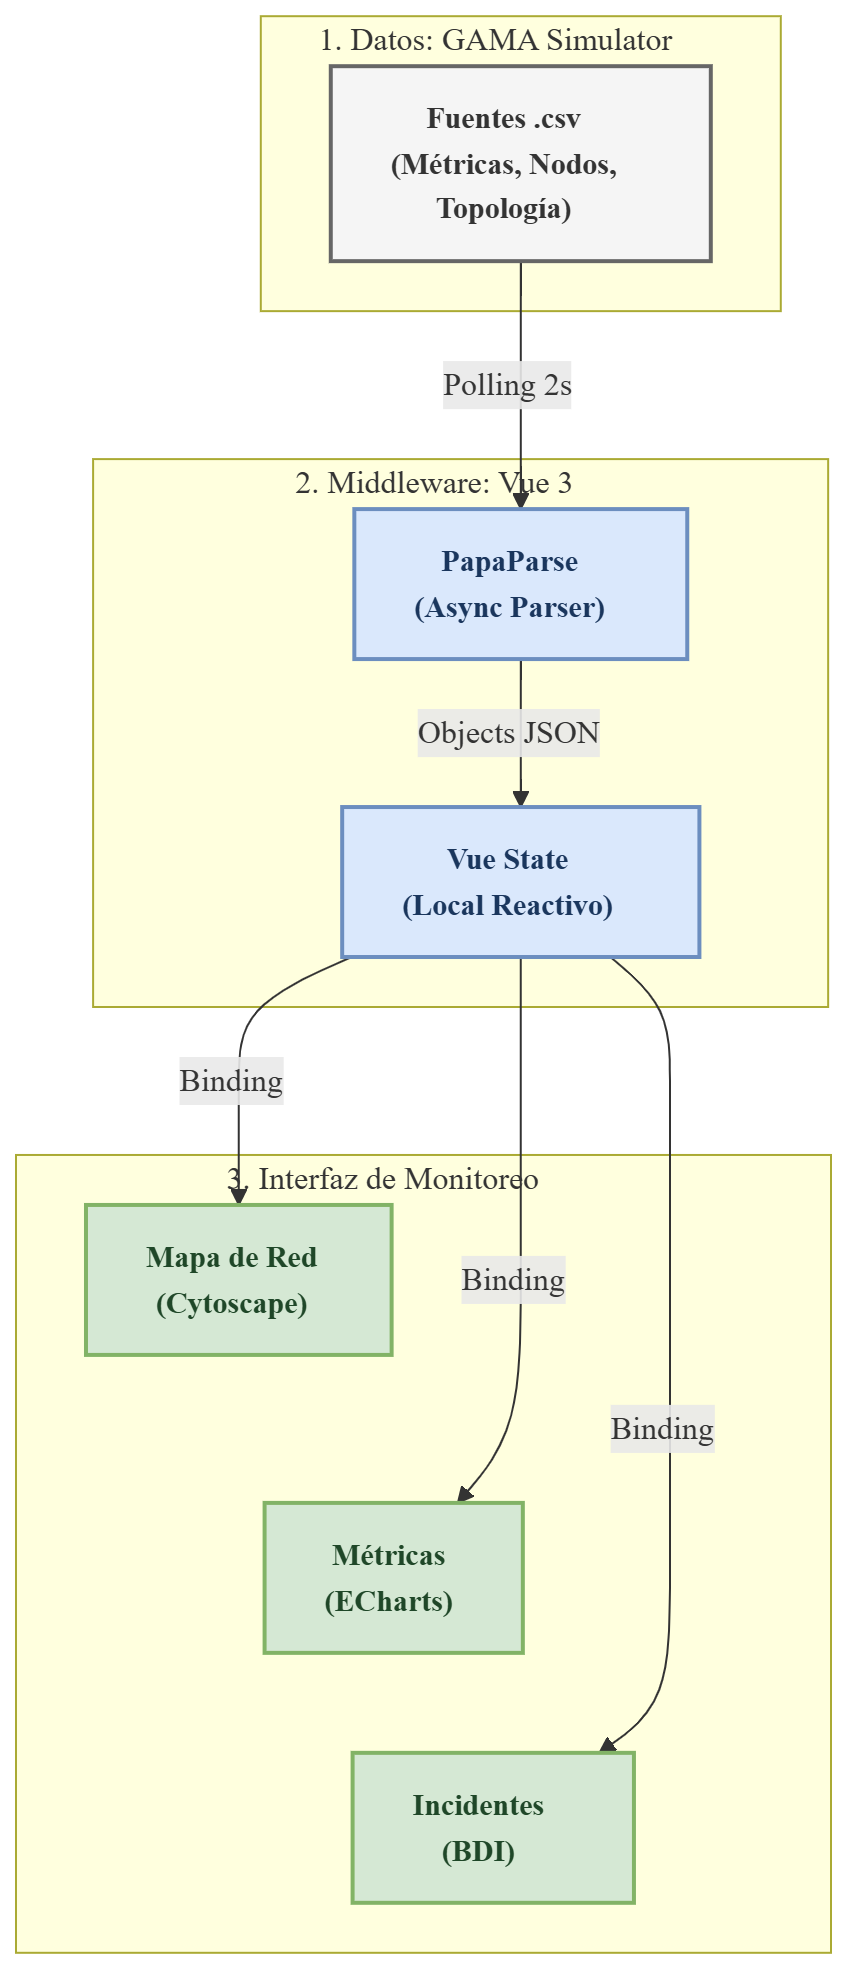
\includegraphics[width=0.90\columnwidth,height=16.9cm,keepaspectratio]{assets/curvas_simulacion1.png}
\caption{Gráficas temporales de hosts infectados, patch level e intenciones BDI en el dashboard Vue 3.}
\label{fig:curvas_dashboard}
\end{figure}